%%%%%%%%%%%%%%%%%%%%%%%%%%%%%%%%%%%%%%%%%%%%%%%%%%%%%%%%%%%%%%%%%%%%%%%%%%%%%%%%%%
\begin{frame}[fragile]\frametitle{}
\begin{center}
{\Large Samadhi Paad समाधिपाद}
\end{center}
\end{frame}


%%%%%%%%%%%%%%%%%%%%%%%%%%%%%%%%%%%%%%%%%%%%%%%%%%%%%%%%%%%
\begin{frame}[fragile]\frametitle{Introduction}


	\begin{itemize}
	\item Samadhi refers to a blissful state of existence that is believed to be even beyond mind and meditation.
	\item In this chapter, the author describes yoga and then our true nature and then he instructs the means to attain Samadhi. 
	\item Patanjali begins this chapter with a definition of yoga.
	\item He lists the obstacles we may encounter to attaining mental silence. 
	\item But, having overcome such obstacles, he explains what it is like when we have achieved mental silence as well.
	\end{itemize}

\tiny{(Ref: Basic Introduction of Patanjali Yoga Sutras – The Best Knowledge for Yogis - Yoga Moha)}

\end{frame}

%%%%%%%%%%%%%%%%%%%%%%%%%%%%%%%%%%%%%%%%%%%%%%%%%%%%%%%%%%%
\begin{frame}[fragile]\frametitle{Types of Samadhi समाधी}

\begin{center}
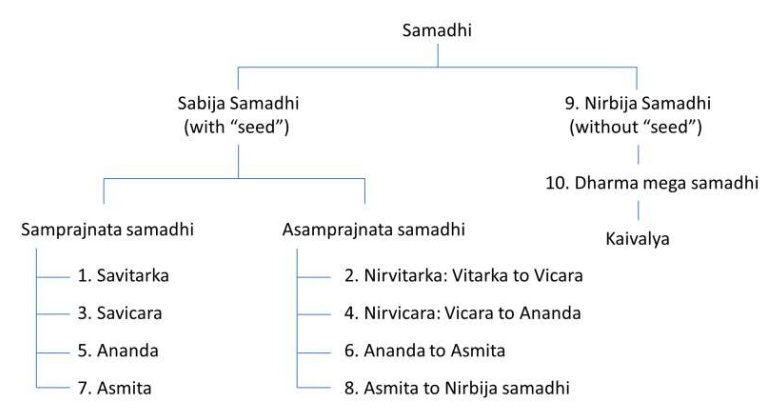
\includegraphics[width=\linewidth,keepaspectratio]{yog37}

\end{center}

  
  \tiny{(Ref: Patanjali Yoga Darshan- For AYUSH YOGA EXAM- Deepak D.Khaire)}

\end{frame}


%%%%%%%%%%%%%%%%%%%%%%%%%%%%%%%%%%%%%%%%%%%%%%%%%%%%%%%%%%%
\begin{frame}[fragile]\frametitle{The Beginning}

अथ योग अनुशासनम् 1.01

	\begin{itemize}
	\item अथ primarily means `now' has many levels of meanings.
	\begin{itemize}
	\item You have done lots of reading, getting knowledge, NOW, lets practice Yog
	\item You have been coming from different evolutionary paths, NOW you are eligible to do Yog
	\item अनुशासनम् means discipline. अनु means following. Now follow the Yog tradition. Meaning Yog was known before (like in Gita), NOW its time to continue/follow it.
	\end{itemize}	
	\end{itemize}

\end{frame}


%%%%%%%%%%%%%%%%%%%%%%%%%%%%%%%%%%%%%%%%%%%%%%%%%%%%%%%%%%%
\begin{frame}[fragile]\frametitle{Definition of Yog}

योग: चित्तवृत्ति निरोध: १.०२

	\begin{itemize}
	\item Yog is complete cessation/stilling of perturbations of mind
	\item चित (chit): to enlighten to know, to make aware (जाणणे/जानना)
	\item चित्त (chitta): the enlightened, all inclusive term, different faculties of mind.
	\end{itemize}

\end{frame}


%%%%%%%%%%%%%%%%%%%%%%%%%%%%%%%%%%%%%%%%%%%%%%%%%%%%%%%%%%%
\begin{frame}[fragile]\frametitle{चित्त}

	\begin{itemize}
	\item अन्त:करण : मन, बुद्धि, अहंकार, चित्त
	\item Chitta is like a river, flowing in two opposite directions: worldliness to/from Kaivalya कैवल्य (व्यास भाष्य)
	\item Levels of Chitta:
		\begin{itemize}
		\item मूढ चित्त  Dull, intertial, Tamas तमस
		\item क्षिप्त चित्त  Restless, distracted, Rajas  रजस
		\item विक्षिप्त चित्त Sometimes steady Sattva सत्व
		\item एकाग्र चित्त Focused
		\item निरुद्ध चित्त Restricted
		
		\end{itemize}	
	\end{itemize}

\end{frame}

%%%%%%%%%%%%%%%%%%%%%%%%%%%%%%%%%%%%%%%%%%%%%%%%%%%%%%%%%%%
\begin{frame}[fragile]\frametitle{Essence of Yog}

\begin{sanskrit}
योग: चित्तवृत्ति निरोध: १.०२

तदा द्रष्टु: स्वरुपे अवस्थानम् १.०३

वृत्ति सारुप्यं इतरत्र १.०४
\end{sanskrit}


	\begin{itemize}
	\item Yog is complete cessation/stilling of perturbations of mind
	\item Once the stilling happens, Then the seer (Purush, पुरुष ) gets to see his own true nature.
	\item Till that time, there is a continual identification with vruttis वृत्ति like reflection of the moon in the lake.
	\item Essence of Yog: still the mind-lake, to see the true bottom.
	\end{itemize}

\end{frame}

%%%%%%%%%%%%%%%%%%%%%%%%%%%%%%%%%%%%%%%%%%%%%%%%%%%%%%%%%%%
\begin{frame}[fragile]\frametitle{वृत्ति}

	\begin{itemize}
	\item वृत्तय: पञ्चतय्य: क्लिष्टा अक्लिष्टा १.०५
	\item 5 types of vruttis : painful/complicated and not complicated
	\item प्रमाणं विपर्यय विकल्प निद्रा स्मृतय: १.०६
		\begin{itemize}
		\item प्रमाणं : यथार्थ ज्ञान : correct knowledge with right perception
		\item विपर्यय : भ्रामक ज्ञान : False knowledge
		\item विकल्प : काल्पनिक ज्ञान : Imaginary knowledge
		\item निद्रा : अभाव ज्ञान : Lack of knowledge
		\item स्मृति : Memory
		
		\end{itemize}	
	\end{itemize}

\end{frame}

%%%%%%%%%%%%%%%%%%%%%%%%%%%%%%%%%%%%%%%%%%%%%%%%%%%%%%%%%%%
\begin{frame}[fragile]\frametitle{चित्त वृत्ति}

\begin{sanskrit}
प्रत्यक्ष अनुमान आगम: प्रमाणानि १.०७

विपर्यय: मिथ्या ज्ञानम् अतद् रूप प्रतिष्ठम् १.०८

शब्द ज्ञान अनुपाति वस्तु शून्यो विकल्प: १.०९
\end{sanskrit}


	\begin{itemize}
	\item Correct knowledge is obtained through direct perception
	\item Incorrect knowledge is based on false perception, eg rope looks like a snake in the dark
	\item Verbal knowledge which does not have actual object is imaginary knowledge eg horn of rabbit
	\end{itemize}

\end{frame}
